\section{Literature Review}
\subsection{Existing relative researches and solutions}
There are several researches introduced Reinforcement Learning framework to generate an optimal pulse sequence to achieve a consistent images compared with a pre-designed pulse sequence. Based on the sequence they focused, researches can be divided into two main part: gradient echo (GE) sequence generator and adiofrequency wave (RF) generator. 
\\\\
As illustrated in Figure \ref{schematic}, \citet{0438} generated the gradient-echo sequence $X(t)$ by an agent from a distribution $p(X)$ that modeled by a dependent Gaussian process. The interaction between the action $X(t)$ and the environment was simulated by a Bayesian Neural Network $f:X(t) \rightarrow y$, where $y$ represented the score of the predicted signal compared with the target signal. To address the exploitation and exploration dilemma, the next predicted set of pulse sequences $X^*$ was proposed by $p\left(f \mid y_t, X_{t+1}\right)$ by maximizing the acquisition function $u_t(X)$.

\begin{figure}[ht]
    \centering
    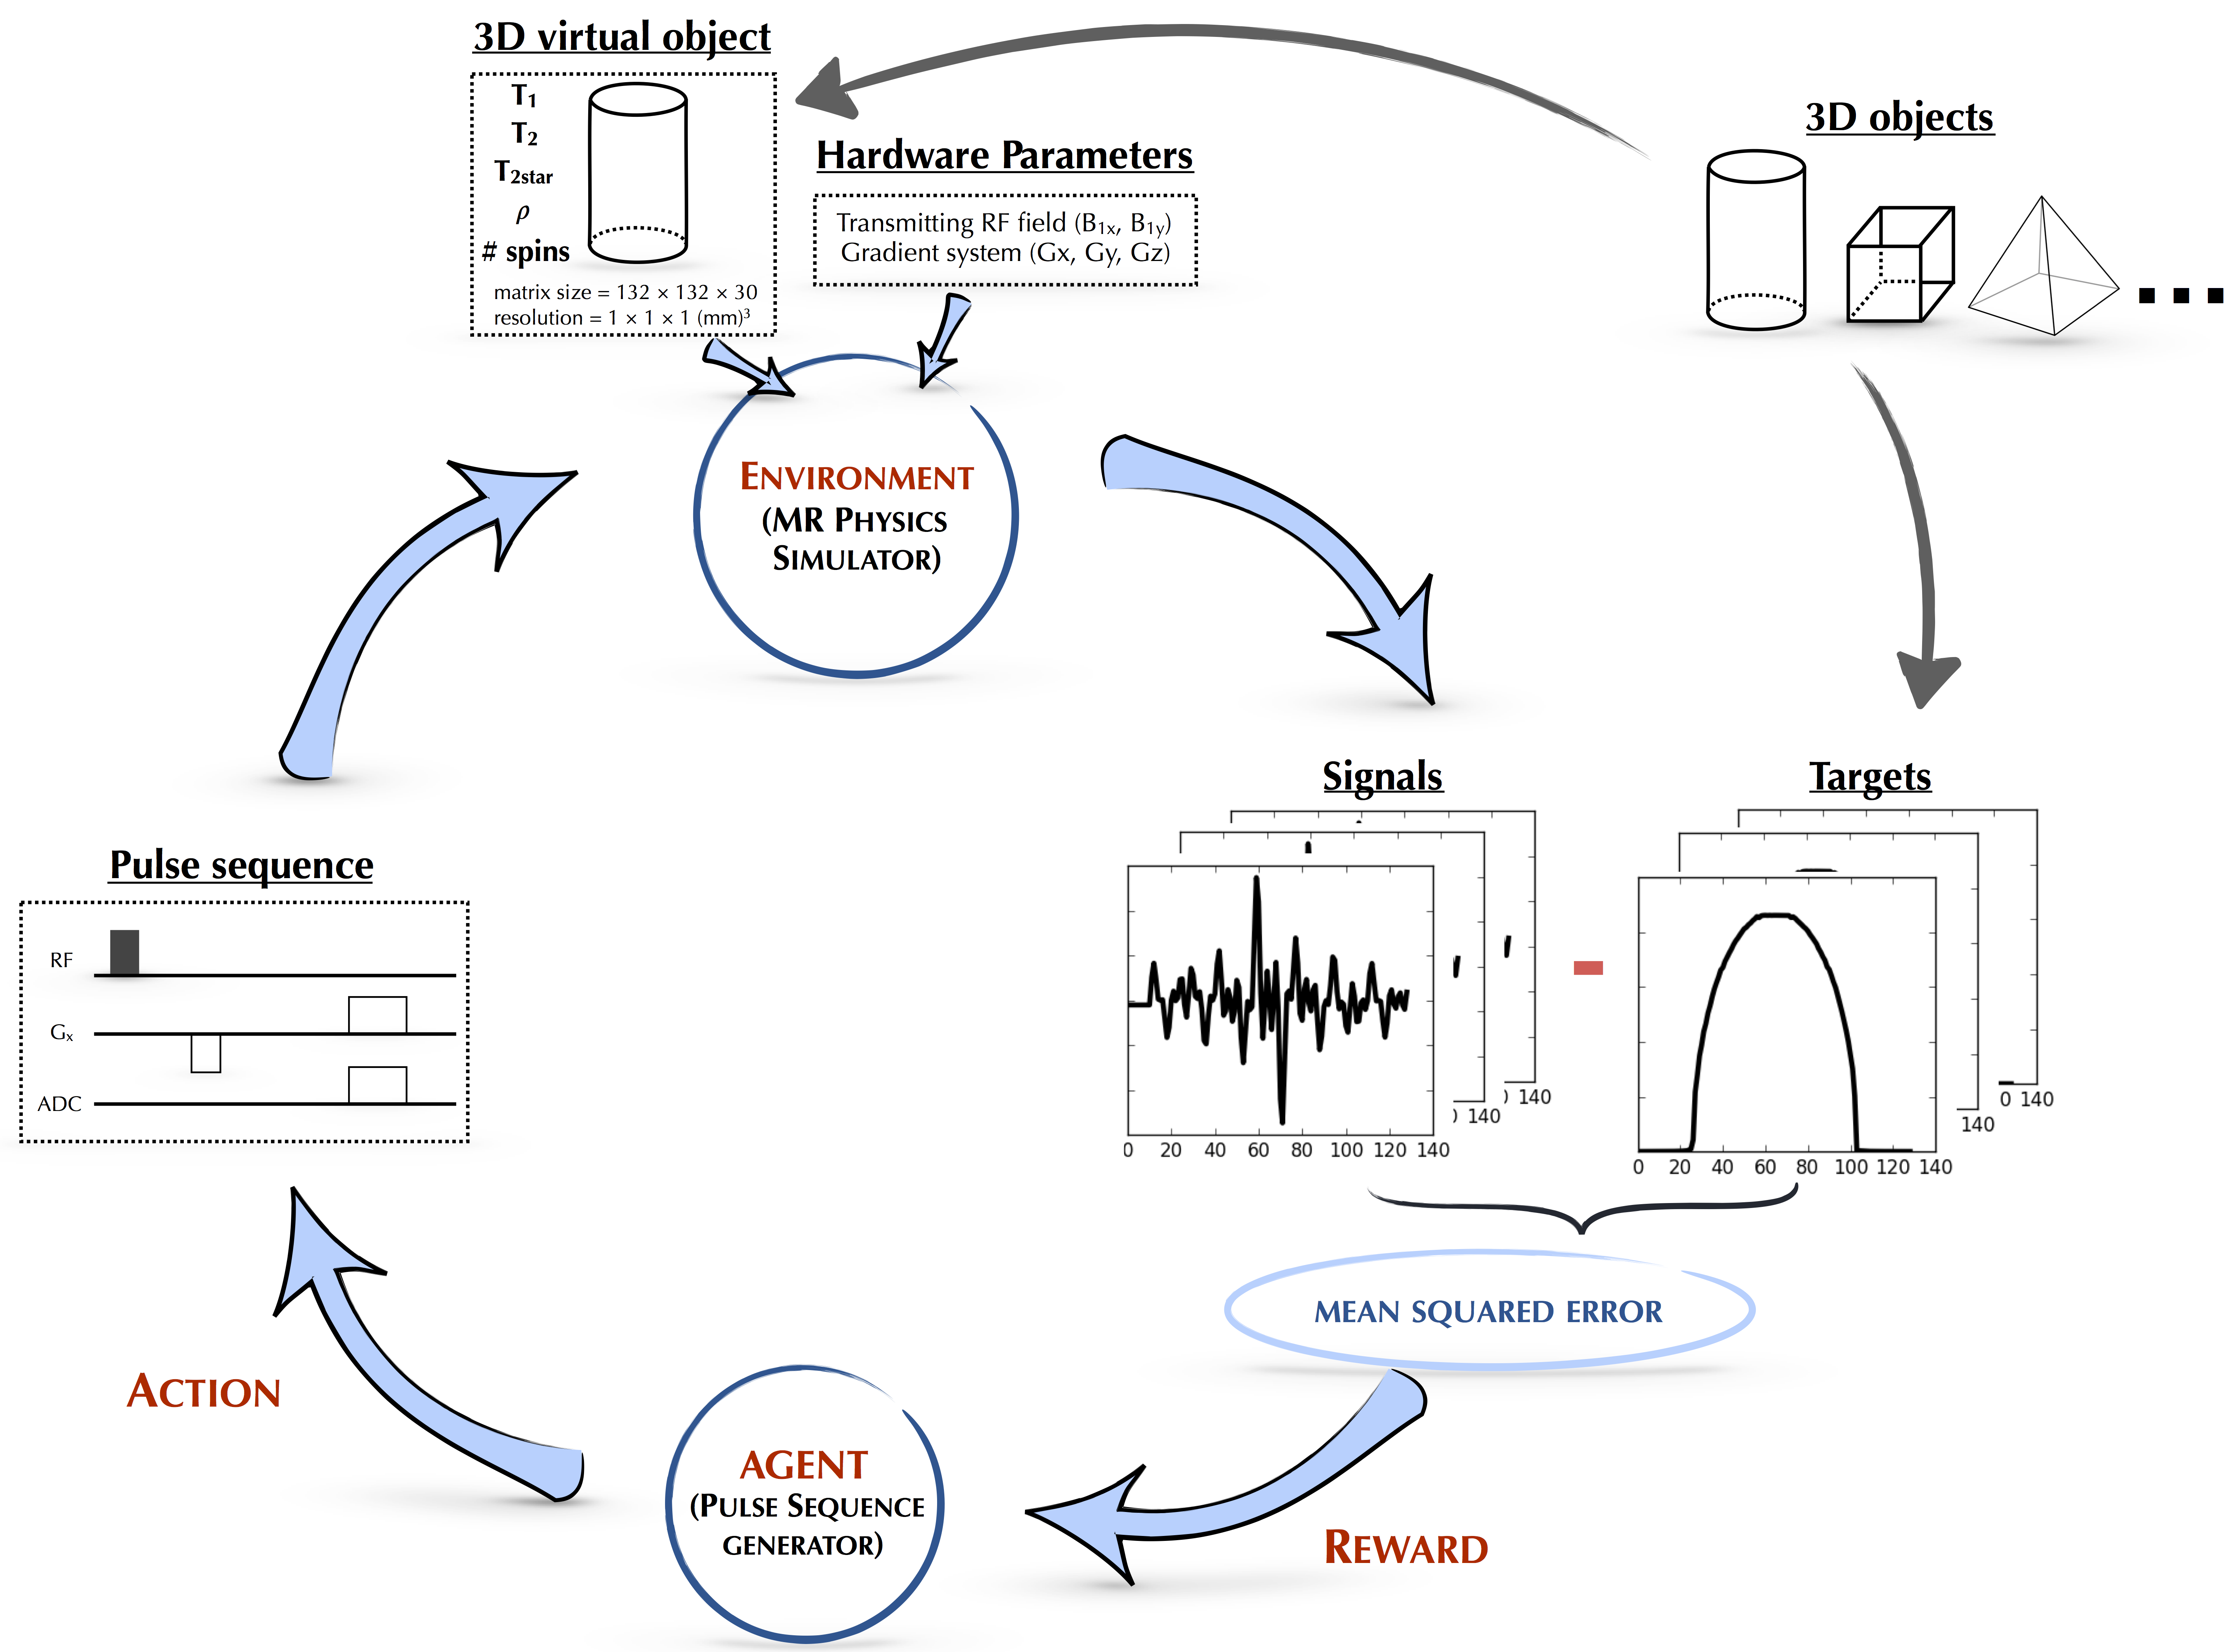
\includegraphics[scale=0.6]{schematic.png}
    \caption{Schematic of the AUTOSEQ Reinforcement Learning framework \citep{0438}.}
    \label{schematic}
\end{figure}

\subsection{Limitations of the current state of the art}
Though the preceding works have yielded satisfactory outcomes in addressing their respective problems, the empirical validation of the generalizability of RL models remains a critical concern. In an attempt to provide empirical evidence, \citet{0438} conducted experiments under a 1-D condition and examined specific constraints on a single $G_x$ but no conclusive evidence was presented regarding the generalizability of RL frameworks in more complex scenarios like higher dimensions or more sophisticated constraints. Additionally, a valuable research problem is the capacity to utilize the RL framework to design a comprehensive pulse sequence that encode radiofrequency (RF) waves and gradient echo sequences together.